%%%%%%%%%%%%%%%%%%%%%%%%%%%%%%%%%%%%%%%%%%%%%%%%%%%%%%%%%%%%%%%%%%%%%%%%%%%%%%%%%%%%
% Template for STAT 548 Qualifying Paper Report
% Author: Ben Bloem-Reddy <benbr@stat.ubc.ca>
% Revised: Daniel J. McDonald <daniel@stat.ubc.ca>
% Date: 20 August 2022
%%%%%%%%%%%%%%%%%%%%%%%%%%%%%%%%%%%%%%%%%%%%%%%%%%%%%%%%%%%%%%%%%%%%%%%%%%%%%%%%%%%%

% Note: You will get an empty bibliography warning when compiling until you include a citation.
\documentclass[12pt]{article}
\usepackage[autonum]{shortex}
% header.tex
% this is where you load pacakges, specify custom formats, etc.

\usepackage[margin=1in,footskip=25pt]{geometry} 
% \usepackage{changepage}
\usepackage{amsmath,amsthm,amssymb,amsfonts}
\usepackage{mathtools}
% enumitem for custom lists
\usepackage{enumitem}
% Load dsfont this to get proper indicator function (bold 1) with \mathds{1}:
\usepackage{dsfont}
\usepackage{centernot}

\usepackage[usenames,dvipsnames]{xcolor}

% set up commenting code (I will use this during marking)
\definecolor{CommentColor}{rgb}{0,.50,.50}
\newcounter{margincounter}
\newcommand{\displaycounter}{{\arabic{margincounter}}}
\newcommand{\incdisplaycounter}{{\stepcounter{margincounter}\arabic{margincounter}}}
\newcommand{\COMMENT}[1]{\textcolor{CommentColor}{$\,^{(\incdisplaycounter)}$}\marginpar{\scriptsize\textcolor{CommentColor}{ {\tiny $(\displaycounter)$} #1}}}

\usepackage{appendix}

% set up graphics
\usepackage{graphicx}
\DeclareGraphicsExtensions{.pdf,.png,.jpg}
\graphicspath{ {fig/} }


\usepackage[sort&compress,round]{natbib}

%%%%%%%%%%%%%%%%%%%%%%%%%%%%%%%%%%%%%%%%%%%%%%%%%%%%%%%%%%%%%%%%%%%%%%%%%%%%%%%%%%%%
% most other packages you might use should be loaded before hyperref
%%%%%%%%%%%%%%%%%%%%%%%%%%%%%%%%%%%%%%%%%%%%%%%%%%%%%%%%%%%%%%%%%%%%%%%%%%%%%%%%%%%%

% Set up hyperlinks:
\definecolor{RefColor}{rgb}{0,0,.65}
\usepackage[colorlinks,linkcolor=RefColor,citecolor=RefColor,urlcolor=RefColor]{hyperref}

\usepackage[capitalize]{cleveref}
\crefname{appsec}{Appendix}{Appendices} % you can tell cleveref what to call things
% defs.tex
% this is where you define custom notation, commands, etc.


%%
% full alphabets of different styles
%%

% bf series
\def\bfA{\mathbf{A}}
\def\bfB{\mathbf{B}}
\def\bfC{\mathbf{C}}
\def\bfD{\mathbf{D}}
\def\bfE{\mathbf{E}}
\def\bfF{\mathbf{F}}
\def\bfG{\mathbf{G}}
\def\bfH{\mathbf{H}}
\def\bfI{\mathbf{I}}
\def\bfJ{\mathbf{J}}
\def\bfK{\mathbf{K}}
\def\bfL{\mathbf{L}}
\def\bfM{\mathbf{M}}
\def\bfN{\mathbf{N}}
\def\bfO{\mathbf{O}}
\def\bfP{\mathbf{P}}
\def\bfQ{\mathbf{Q}}
\def\bfR{\mathbf{R}}
\def\bfS{\mathbf{S}}
\def\bfT{\mathbf{T}}
\def\bfU{\mathbf{U}}
\def\bfV{\mathbf{V}}
\def\bfW{\mathbf{W}}
\def\bfX{\mathbf{X}}
\def\bfY{\mathbf{Y}}
\def\bfZ{\mathbf{Z}}

% bb series
\def\bbA{\mathbb{A}}
\def\bbB{\mathbb{B}}
\def\bbC{\mathbb{C}}
\def\bbD{\mathbb{D}}
\def\bbE{\mathbb{E}}
\def\bbF{\mathbb{F}}
\def\bbG{\mathbb{G}}
\def\bbH{\mathbb{H}}
\def\bbI{\mathbb{I}}
\def\bbJ{\mathbb{J}}
\def\bbK{\mathbb{K}}
\def\bbL{\mathbb{L}}
\def\bbM{\mathbb{M}}
\def\bbN{\mathbb{N}}
\def\bbO{\mathbb{O}}
\def\bbP{\mathbb{P}}
\def\bbQ{\mathbb{Q}}
\def\bbR{\mathbb{R}}
\def\bbS{\mathbb{S}}
\def\bbT{\mathbb{T}}
\def\bbU{\mathbb{U}}
\def\bbV{\mathbb{V}}
\def\bbW{\mathbb{W}}
\def\bbX{\mathbb{X}}
\def\bbY{\mathbb{Y}}
\def\bbZ{\mathbb{Z}}

% cal series
\def\calA{\mathcal{A}}
\def\calB{\mathcal{B}}
\def\calC{\mathcal{C}}
\def\calD{\mathcal{D}}
\def\calE{\mathcal{E}}
\def\calF{\mathcal{F}}
\def\calG{\mathcal{G}}
\def\calH{\mathcal{H}}
\def\calI{\mathcal{I}}
\def\calJ{\mathcal{J}}
\def\calK{\mathcal{K}}
\def\calL{\mathcal{L}}
\def\calM{\mathcal{M}}
\def\calN{\mathcal{N}}
\def\calO{\mathcal{O}}
\def\calP{\mathcal{P}}
\def\calQ{\mathcal{Q}}
\def\calR{\mathcal{R}}
\def\calS{\mathcal{S}}
\def\calT{\mathcal{T}}
\def\calU{\mathcal{U}}
\def\calV{\mathcal{V}}
\def\calW{\mathcal{W}}
\def\calX{\mathcal{X}}
\def\calY{\mathcal{Y}}
\def\calZ{\mathcal{Z}}


%%%%%%%%%%%%%%%%%%%%%%%%%%%%%%%%%%%%%%%%%%%%%%%%%%%%%%%%%%
% text short-cuts
\def\iid{i.i.d.\ } %i.i.d.
\def\ie{i.e.\ }
\def\eg{e.g.\ }
\def\Polya{P\'{o}lya\ }
%%%%%%%%%%%%%%%%%%%%%%%%%%%%%%%%%%%%%%%%%%%%%%%%%%%%%%%%%%

%%%%%%%%%%%%%%%%%%%%%%%%%%%%%%%%%%%%%%%%%%%%%%%%%%%%%%%%%%
% quasi-universal probabilistic and mathematical notation
% my preferences (modulo publication conventions, and clashes like random vectors):
%   vectors: bold, lowercase
%   matrices: bold, uppercase
%   operators: blackboard (e.g., \mathbb{E}), uppercase
%   sets, spaces: calligraphic, uppercase
%   random variables: normal font, uppercase
%   deterministic quantities: normal font, lowercase
%%%%%%%%%%%%%%%%%%%%%%%%%%%%%%%%%%%%%%%%%%%%%%%%%%%%%%%%%%

% operators
\def\P{\bbP} %fundamental probability
\def\E{\bbE} %expectation

\newcommand{\Expect}[1]{\E \left{ #1\right}}
% conditional expectation
\DeclarePairedDelimiterX\bigCond[2]{[}{]}{#1 \;\delimsize\vert\; #2}
\newcommand{\conditional}[3][]{\E_{#1}\bigCond*{#2}{#3}}
\def\Law{\mathcal{L}} %law; this is by convention in the literature
\def\indicator{\mathds{1}} % indicator function

% norms
\newcommand{\norm}[1]{\left\lVert #1 \right\rVert}

% binary relations
\def\condind{{\perp\!\!\!\perp}} %independence/conditional independence
\def\equdist{\stackrel{\text{\rm\tiny d}}{=}} %equal in distribution
\def\equas{\stackrel{\text{\rm\tiny a.s.}}{=}} %euqal amost surely
\def\simiid{\sim_{\mbox{\tiny iid}}} %sampled i.i.d

% common vectors and matrices
\def\onevec{\mathbf{1}}
\def\iden{\mathbf{I}} % identity matrix
\def\supp{\text{\rm supp}}

% misc
% floor and ceiling
\DeclarePairedDelimiter{\ceilpair}{\lceil}{\rceil}
\DeclarePairedDelimiter{\floor}{\lfloor}{\rfloor}
\newcommand{\argdot}{{\,\vcenter{\hbox{\tiny$\bullet$}}\,}} %generic argument dot
%%%%%%%%%%%%%%%%%%%%%%%%%%%%%%%%%%%%%%%%%%%%%%%%%%%%%%%%%%

%%%%%%%%%%%%%%%%%%%%%%%%%%%%%%%%%%%%%%%%%%%%%%%%%%%%%%%%%%
%% some distributions
% continuous
\def\UnifDist{\text{\rm Unif}}
\def\BetaDist{\text{\rm Beta}}
\def\ExpDist{\text{\rm Exp}}
\def\GammaDist{\text{\rm Gamma}}
\def\NormalDist{\text{\rm Normal}}


% discrete
\def\BernDist{\text{\rm Bernoulli}}
\def\BinomDist{\text{\rm Binomial}}
\def\PoissonDist{\text{\rm Poisson}}
%%%%%%%%%%%%%%%%%%%%%%%%%%%%%%%%%%%%%%%%%%%%%%%%%%%%%%%%%%

%%%%%%%%%%%%%%%%%%%%%%%%%%%%%%%%%%%%%%%%%%%%%%%%%%%%%%%%%%
% Project-specific notation should go here
% (Because it's at the end of the file, it can overwrite anything that came before.)



%%%%%%%%%%%%%%%%%%%%%%%%%%%%%%%%%%%%%%%%%%%%%%%%%%%%%%%%%%



%%%%%%%%%%%%%%%%%%%%%%%%%%%%%%%%%%%%%%%%%%%%%%%%%%%%%%%%%%%%%%%%%%%%%%%%%%%%%%%%%

% your title/author/date information go here
\title{Qualifying Paper Report for Data Fission: Splitting A Single Data Point} % replace with your title, a meaningful title
\author{Naitong Chen} % replace with your name
\date{\today} % replace with your submission date


% start of document
\begin{document}

\maketitle

\section{Problem Definition}\label{sec:problem_def}
Given a dataset $(X_i)_{i=1}^n \distiid \pi_\theta$, with $\pi_\theta$ being a distribution from the exponential family whose parameter $\theta$ is of interest. We decompose each $X_i$ to $f(X_i)$ and $g(X_i)$ such that both parts contain information about $\theta$, and there exists some function $h$ such that $X_i = h(f(X_i), g(X_i))$ satisfying either of the two properties:
\begin{itemize}
\item (P1): $f(X_i)$ and $g(X_i)$ are independent with known distributions (up to unknown $\theta$);
\item (P2): $f(X_i)$ has a known marginal distribution and $g(X_i)$ has a known conditional distribution given $f(X_i)$ (up to unknown $\theta$).
\newline $ $
\color{red}
Typos and missing terms in the proof of the original paper. See \cref{thm:conjugacy} for a modified version.
\color{black}
\end{itemize}
\section{Significance}
As mentioned in the previous section, data splitting may not always be an ideal framework for selective inference. As a result, there has been a variety of alternative procedures developed. For example, the idea of introducing external randomness to derive valid inference procedures rather than randomly partitioning the data is explored in \cite{tian2018selective} and \cite{rasines2021splitting}. In the Gaussian example discussed in \cref{sec:problem_def}, their approach is equivalent to setting $f_\tau(X) = X+\tau Z$ and $g_\tau(X) = X$. The finite sample distribution of $g_\tau(X) \given f_\tau(X)$ is also known when the data are Gaussian. However, if we move beyond Gaussianity, the distribution of $g_\tau(X) \given f_\tau(X)$ is only known asymptotically. In these cases, using this asymptotic result may hinder the performance of selective inference, particularly in the small sample setting, which is one situation where data splitting struggles that we would like to address. Another approach developed in \cite{fithian2014optimal} is data carving. Data carving performs model selection using some fixed model selection procedure $S$ on the original dataset. By denoting the selected model as $S(X)$, we then conduct inference on $X$ conditioned on $S(X)$. Instead of injecting external randomness, data carving performs inference using the ``leftover information'' from the selection step obtained through conditioning. However, since the distribution of $X\given S(X)$ depends on the selection procedure $S$, practitioners are limited to choices of $S$ such that $X\given S(X)$ can be obtained either analytically or numerically. Examples include LASSO \citep{lee2016exact} and step-wise regression \citep{tibshirani2016exact}.

Data fission combines the advantages of both approaches. Similar to the approach in \cite{tian2018selective} and \cite{rasines2021splitting}, we create two slightly perturbed datasets, $f_\tau(X)$ and $g_\tau(X)$, both of which are of the same size of the original data. This is done by injecting external randomness ($Z$) to the original data at hand. Here the distribution of $Z$ and the perturbations are carefully constructed so that both the finite sample marginal distribution of $f_\tau(X)$ and conditional distribution $g_\tau(X)\given f_\tau(X)$ are known analytically. Subsequently, we conduct inference under $g_\tau(X)\given f_\tau(X)$, which is similar in spirit to data carving in terms of taking advantage of the ``leftover information''. It is worth noting that, by cleverly leveraging the mechanism of conjugate distributions, which \cite{leiner2022data} terms ``conjugate prior reversal'', we can derive data fission procedures for many distributions in the rich exponential family. The conditional distribution used for inference is then available regardless of the choice of the selection algorithm, thus making data fission applicable to a much wider-range of problems than both of the other approaches discussed.

\section{Limitations and challenges}\label{sec:challenge}
Closer inspection of the two data fission examples given in \cref{sec:problem_def} reveals that both the marginal distribution of $f_\tau(X)$ and conditional distribution $f_\tau(X) \given g_\tau(X)$ depend on parameters of the distribution of the original data $X$. In fact, a general assumption of data fission is that the distribution of $X$ needs to be known. This may not be a realstic assumption for many cases in practice. Although \cite{leiner2022data} provides an asymptotic CI for Gaussian linear regression when only a consistent estimator of the variance rather than the true value is available, much of the questions regarding the robustness of data fission to the distribution assumption beyond the Gaussian case remain unexplored. Furthermore, data fission may lead to $f_\tau(X)$ and $g_\tau(X) \given f_\tau(X)$ being under different distribution families than that of $X$. As an example, in \cref{eg:continuous}, with gamma distributed $X$, we have $f_\tau(X)$ following a negative binomial distribution. At the same time, the density of $g_\tau(X)\given f_\tau(X)$ as a function of the original parameter of interest $\theta$ may be highly complex and potentially non-convex. This poses challenges in the inference stage, as discussed in Appendix A.5 of \cite{leiner2022data}. (We provide an instance of this problem in \cref{eg:gam_cont}.) Finally, we note that many data fission procedures will also result in cases where the distributions of $g_\tau(X)\given f_\tau(X)$ depend explicitly on the realized values of $Z$. We more closely explore the effect this has on selective inference in \cref{sec:project}.

Before concluding this section, we note an instance of imprecise notation as well as a possible mistake in \cite{leiner2022data}. Theorem 1 in \cite{leiner2022data} misses the base measure term $m(\cdot)$ in the density function of $X$ and mistakenly uses the raw value of $x$ rather than its natural parameter $\phi(x)$ in both the densities of $X$ and $Z$. Here $\phi$ is the natural parameter transformation function for the distribution of $Z$. For example, for $\distPoiss(\lambda), \phi(\lambda) = \log\lambda$. We present a corrected version of the proof in \cref{thm:conjugacy}. Although the final statement of the theorem remains the same, this notation impreciseness would likely result in incorrect applications of the theorem that may fail to lead us to the desired data fission procedure. Additionally, there seems to be an incorrect data fission procedure derived for gamma distributed data. In particular, the marginal density for $Z$ does not match that of \cref{thm:conjugacy}. We present the details in \cref{eg:discrete}. It is worth noting that even if the result presented in \cite{leiner2022data} were indeed correct, it is still unclear how we can modify the inference step to accommodate this data fission procedure, as the dimension of $Z$ is no longer necessarily the same as $X$.
\section{Paper-specific project}\label{sec:project}
In this section, we compare two of the data fission procedures introduced in \cite{leiner2022data} for Gaussian distributed data against data splitting, in the context of constructing selective CIs in fixed-design linear regression models. Suppose we are given a set of $n$ observations such that for $i\in\{1,\dots,n\}$, $y_i = x_i^\top \beta + \eps_i$,
where for some $p\in\nats$ and known $\sigma>0$, $x_i\in\reals^p$, $\eps_i\distiid \distNorm(0,\sigma^2)$, $\beta\in\reals^p$. Equivalently, we can write $Y_i\distas\distNorm(x_i^\top\beta, \sigma^2)$. Note here we assume that the covariates $x_i$'s are fixed. The goal is to first perform variable selection and then construct CIs for the regression coefficients corresponding to the selected variables. We would like to compare variable selection accuracy as well as inference quality obtained using the following three procedures:
\begin{itemize}
\item Data fission (P1): for each $i\in\{1,\dots,n\}$, and some fixed $\tau\in(0,\infty)$, draw $Z_i\distas\distNorm(0,\sigma^2)$. Let $f_\tau(Y_i) = Y_i + \tau Z_i$, $g_\tau(Y_i) = Y_i - \tau^{-1}Z_i$. Then $f_\tau(Y_i)\indep g_\tau(Y_i)$ and $f_\tau(Y_i)\distas\distNorm(x_i^\top\beta, (1+\tau^2)\sigma^2)$, $g_\tau(Y_i)\distNorm(x_i^\top\beta, (1+\tau^{-2})\sigma^2)$. We use $(f_\tau(Y_i))_{i=1}^n$ for selection and $(g_\tau(Y_i))_{i=1}^n$ for inference.
\item Data fission (P2): for each $i\in\{1,\dots,n\}$, and some fixed $\tau\in(0,\infty)$, draw $Z_i\distas\distNorm(Y_i,\tau\sigma^2)$. Let $f_\tau(Y_i) = Z_i$, $g_\tau(Y_i) = Y_i$. Then $f_\tau(Y_i)\distas\distNorm(x_i^\top\beta, (1+\tau)\sigma^2)$, $g_\tau(Y_i)\given f_\tau(Y_i)\distas\distNorm\left(\frac{\tau}{\tau+1}x_i^\top\beta + \frac{1}{\tau+1}f_\tau(Y_i), \frac{\tau}{\tau+1}\sigma^2\right)$. We use $(f_\tau(Y_i))_{i=1}^n$ for selection and $(g_\tau(Y_i))_{i=1}^n$ for inference.
\item Data splitting: for some fixed $a\in\{\frac{1}{n}, \frac{2}{n}, \dots, 1\}$, randomly draw $an$ observations from $(Y_i)_{i=1}^n$ without replacement. Without loss of generality, denote the first $an$ observations as those that are selected. Use $(Y_i)_{i=1}^{an}$ for selection and $(Y_i)_{i=an+1}^n$ for inference.
\end{itemize}
We begin by observing the three datasets used for the selection step. Both data fission procedures inflate the variance of each observation without changing their underlying means. Data splitting, on the other hand, directly reduces the number of observations without perturbing their underlying distributions. This also introduces uncertainty to the selection step. It is then of interest to compare variable selection accuracies under different sample sizes and the amount of variance inflated. However, recall that from the Fisher information perspective, to make the comparison fair, we set $a = \frac{1}{1+\tau^2}$. As a result, the comparison reduces to be about varying the sample sizes.

We now consider the inference stage. Suppose that the selected model is $M\subset\{1,\dots,p\}$ and that
\[
X_M = \begin{bmatrix} x_{M,1}, \dots, x_{M,n} \end{bmatrix}^\top, \quad Y = \begin{bmatrix} Y_1, \dots, Y_n \end{bmatrix}^\top,
\]
where $x_{M,i}$ is a vector consisting of only the covariates corresponding to the selected features. We then have our ideal target parameter given $M$ as
\[
\beta^\star(M) = \argmin_{\tilde{\beta}} \EE_Y \|Y - X_M\tilde{\beta}\|^2 = (X_M^\top X_M)^{-1}(X_M^\top\mu)
\]
where $\mu = \begin{bmatrix} x_1^\top\beta, \dots, x_n^\top\beta \end{bmatrix}^\top$. However, since we are using slightly perturbed datasets for inference, our estimator $\hbeta(M)$ given the model $M$ for each of the three procedures are
\begin{itemize}
\item Data fission (P1): $\hbeta(M) = (X_M^\top X_M)^{-1}X_M^\top g_\tau(Y) \distas \distNorm(\beta^\star(M), \sigma^2(1+\tau^{-2})(X_M^\top X_M)^{-1})$;
\item Data fission (P2):\\ $\hbeta(M) = (X_M^\top X_M)^{-1}X_M^\top g_\tau(Y) \given f_\tau(Y) \distas \distNorm(\frac{\tau}{\tau+1}\beta^\star(M) + \frac{1}{\tau+1}(X_M^\top X_M)^{-1}X_M^\top f_\tau(Y), \sigma^2\frac{\tau}{\tau+1}(X_M^\top X_M)^{-1})$;
\item Data splitting: $\hbeta(M) = (X_M^\top X_M)^{-1}X_M^\top Y \distas \distNorm(\beta^\star(M), \sigma^2(X_M^\top X_M)^{-1})$.
\end{itemize}
Note that here $f$ and $g$ are applied to each entry of $Y$ and that $X_M$ and $Y$ in data splitting only contains a subset set of $na$ observations.

Looking at the means of each estimator above, both the data fission (P1) and data splitting procedures target $\beta^\star(M)$. On the other hand, the mean of the data fission (P2) estimator depends on the realized values of the external random variable $Z$. Since $\EE[f_\tau(Y)] = \mu$, if we marginalize $f_\tau(Y)$ over the distribution of $\hbeta(M)$, data fission (P2) would also target the ideal parameter $\beta^\star(M)$. However, it is reasonable to suspect that this randomness might affect the quality of inference.

We now look at the variances of the three estimators. Similar to the selection stage, data fission (P1) inflates the variance of $\hbeta(M)$ by a function of $\tau$, and data splitting introduces additional uncertainty by reducing the sample size. However, in data fission (P2), the variance is deflated. Suppose for each $i$, $x_i$ is generated (\iid) by some distribution $\pi$, and assume that for all selected model $M$, $\EE[x_{M,1}x_{M,1}^\top]$ is finite and strictly positive. Then we have
\[
\frac{1}{n}X_M^\top X_M \convp \EE[x_{M,1}x_{M,1}^\top] \implies \left(\frac{1}{n}X_M^\top X_M\right)^{-1} \convp \left( \EE[x_{M,1}x_{M,1}^\top] \right)^{-1} \implies X_M^\top X_M \convp \frac{1}{n}\left( \EE[x_{M,1}x_{M,1}^\top] \right)^{-1}.
\]
Under this assumption, the difference in inference between data splitting and data fission once again comes down to the sample size and the amount of variance inflated or deflated by $\tau$. We therefore set up our simulations as following. Note that this is mostly in line with Section 4 of \cite{leiner2022data}.

We set $a = \frac{1}{2}$ and $\tau=1$ to ensure the amount of Fisher information allocated to the selection stage is the same across all three methods. Let $p=20, \beta_1=\beta_{19}=1$, $\beta_2=\beta_{20}=-1$, and the rest of the entries in $\beta$ be $0$. We also generate the covariates from the standard multivariate Guassian distribution. Note that there is no intercept in our regression model. We then conduct selective inference with varying sample sizes $10, 20, 50, 100$ to evaluate how the performances across all three methods change under different sample sizes. To compare variable selection accuracy, we use as our metrics
\[
\text{power} = \frac{|j\in M: \beta_j \neq 0|}{|j\in [p]: \beta_j \neq 0|}, \quad \text{precision} = \frac{|j\in M: \beta_j \neq 0|}{|M|}.
\]
To compare the quality of inference, we use false coverage rate (FCR), avg. CI length, and avg. L2 error:
\[
\text{FCR} = \frac{|k\in M: [\beta^\star(M)]_k \notin CI_k|}{\max\{|M|, 1\}}, \quad \overline{\text{CI len.}} = \frac{\sum_{k\in M} |\text{CI}_k(2) - \text{CI}_k(1)|}{|M|}, \quad \text{L2 err.} = \frac{\| \beta^\star(M) - \hbeta(M) \|_2^2}{|M|}.
\]
To perform variable selection, we run LASSO using the \texttt{glmnet} package in \texttt{R} with the default settings and the regularization parameter set to \texttt{lambda.1se}. We repeat the above experiments $200$ times and report the median of the above metrics (excluding runs that do not end up selecting any variable in the selection step) in \cref{fig:median}. The same set of plots with the IQR of each metric, along with other details of the experiment is included in \cref{apdx:plots}. Note that since the IQRs have a lot of overlaps, the discussion below is only concerned with the average performance rather than individual trials. The code used to run the simulations and generate the plots can be found at \url{https://github.com/NaitongChen/QP-3}.

\captionsetup[subfigure]{labelformat=empty}
\begin{figure}[ht!]
\centering
\begin{subfigure}[b]{.32\columnwidth} 
    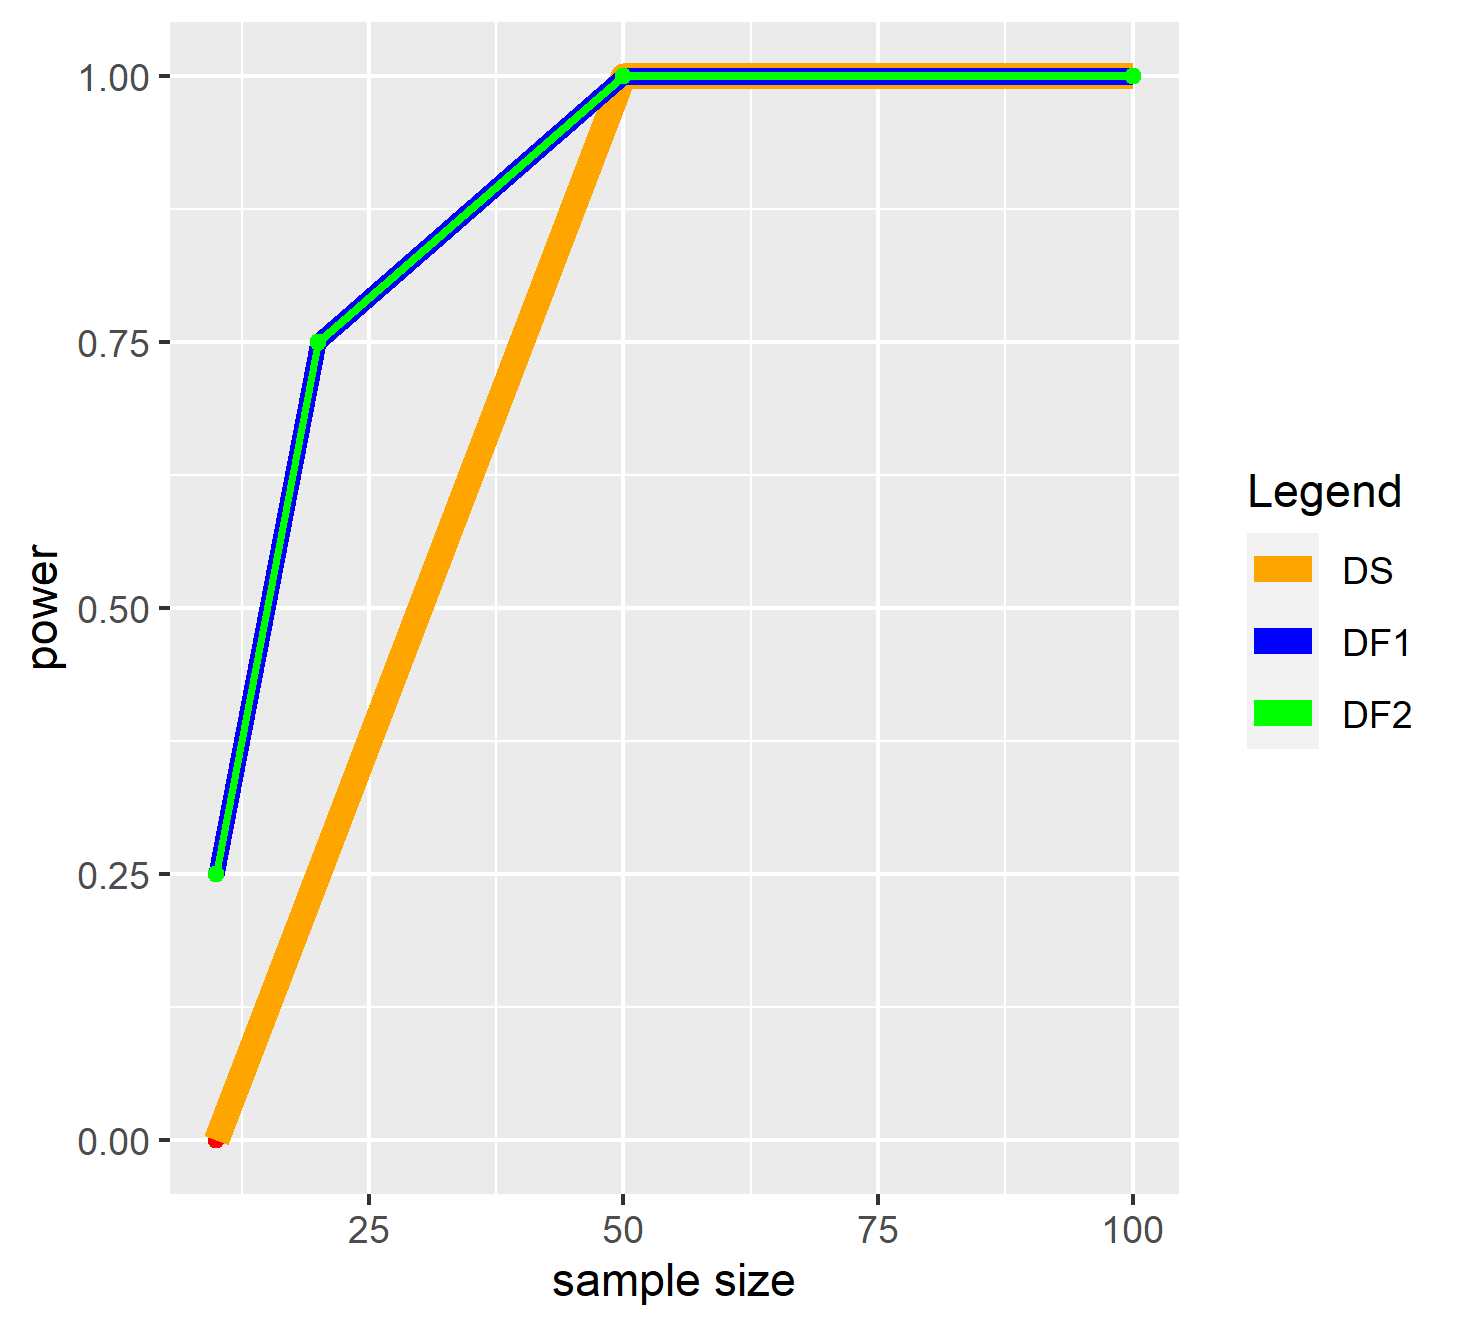
\includegraphics[width=\columnwidth]{../../plot/power_1.png}
    \caption{(a) Power}
    \label{fig:power}
\end{subfigure}
\hfill
\centering
\begin{subfigure}[b]{.32\columnwidth} 
    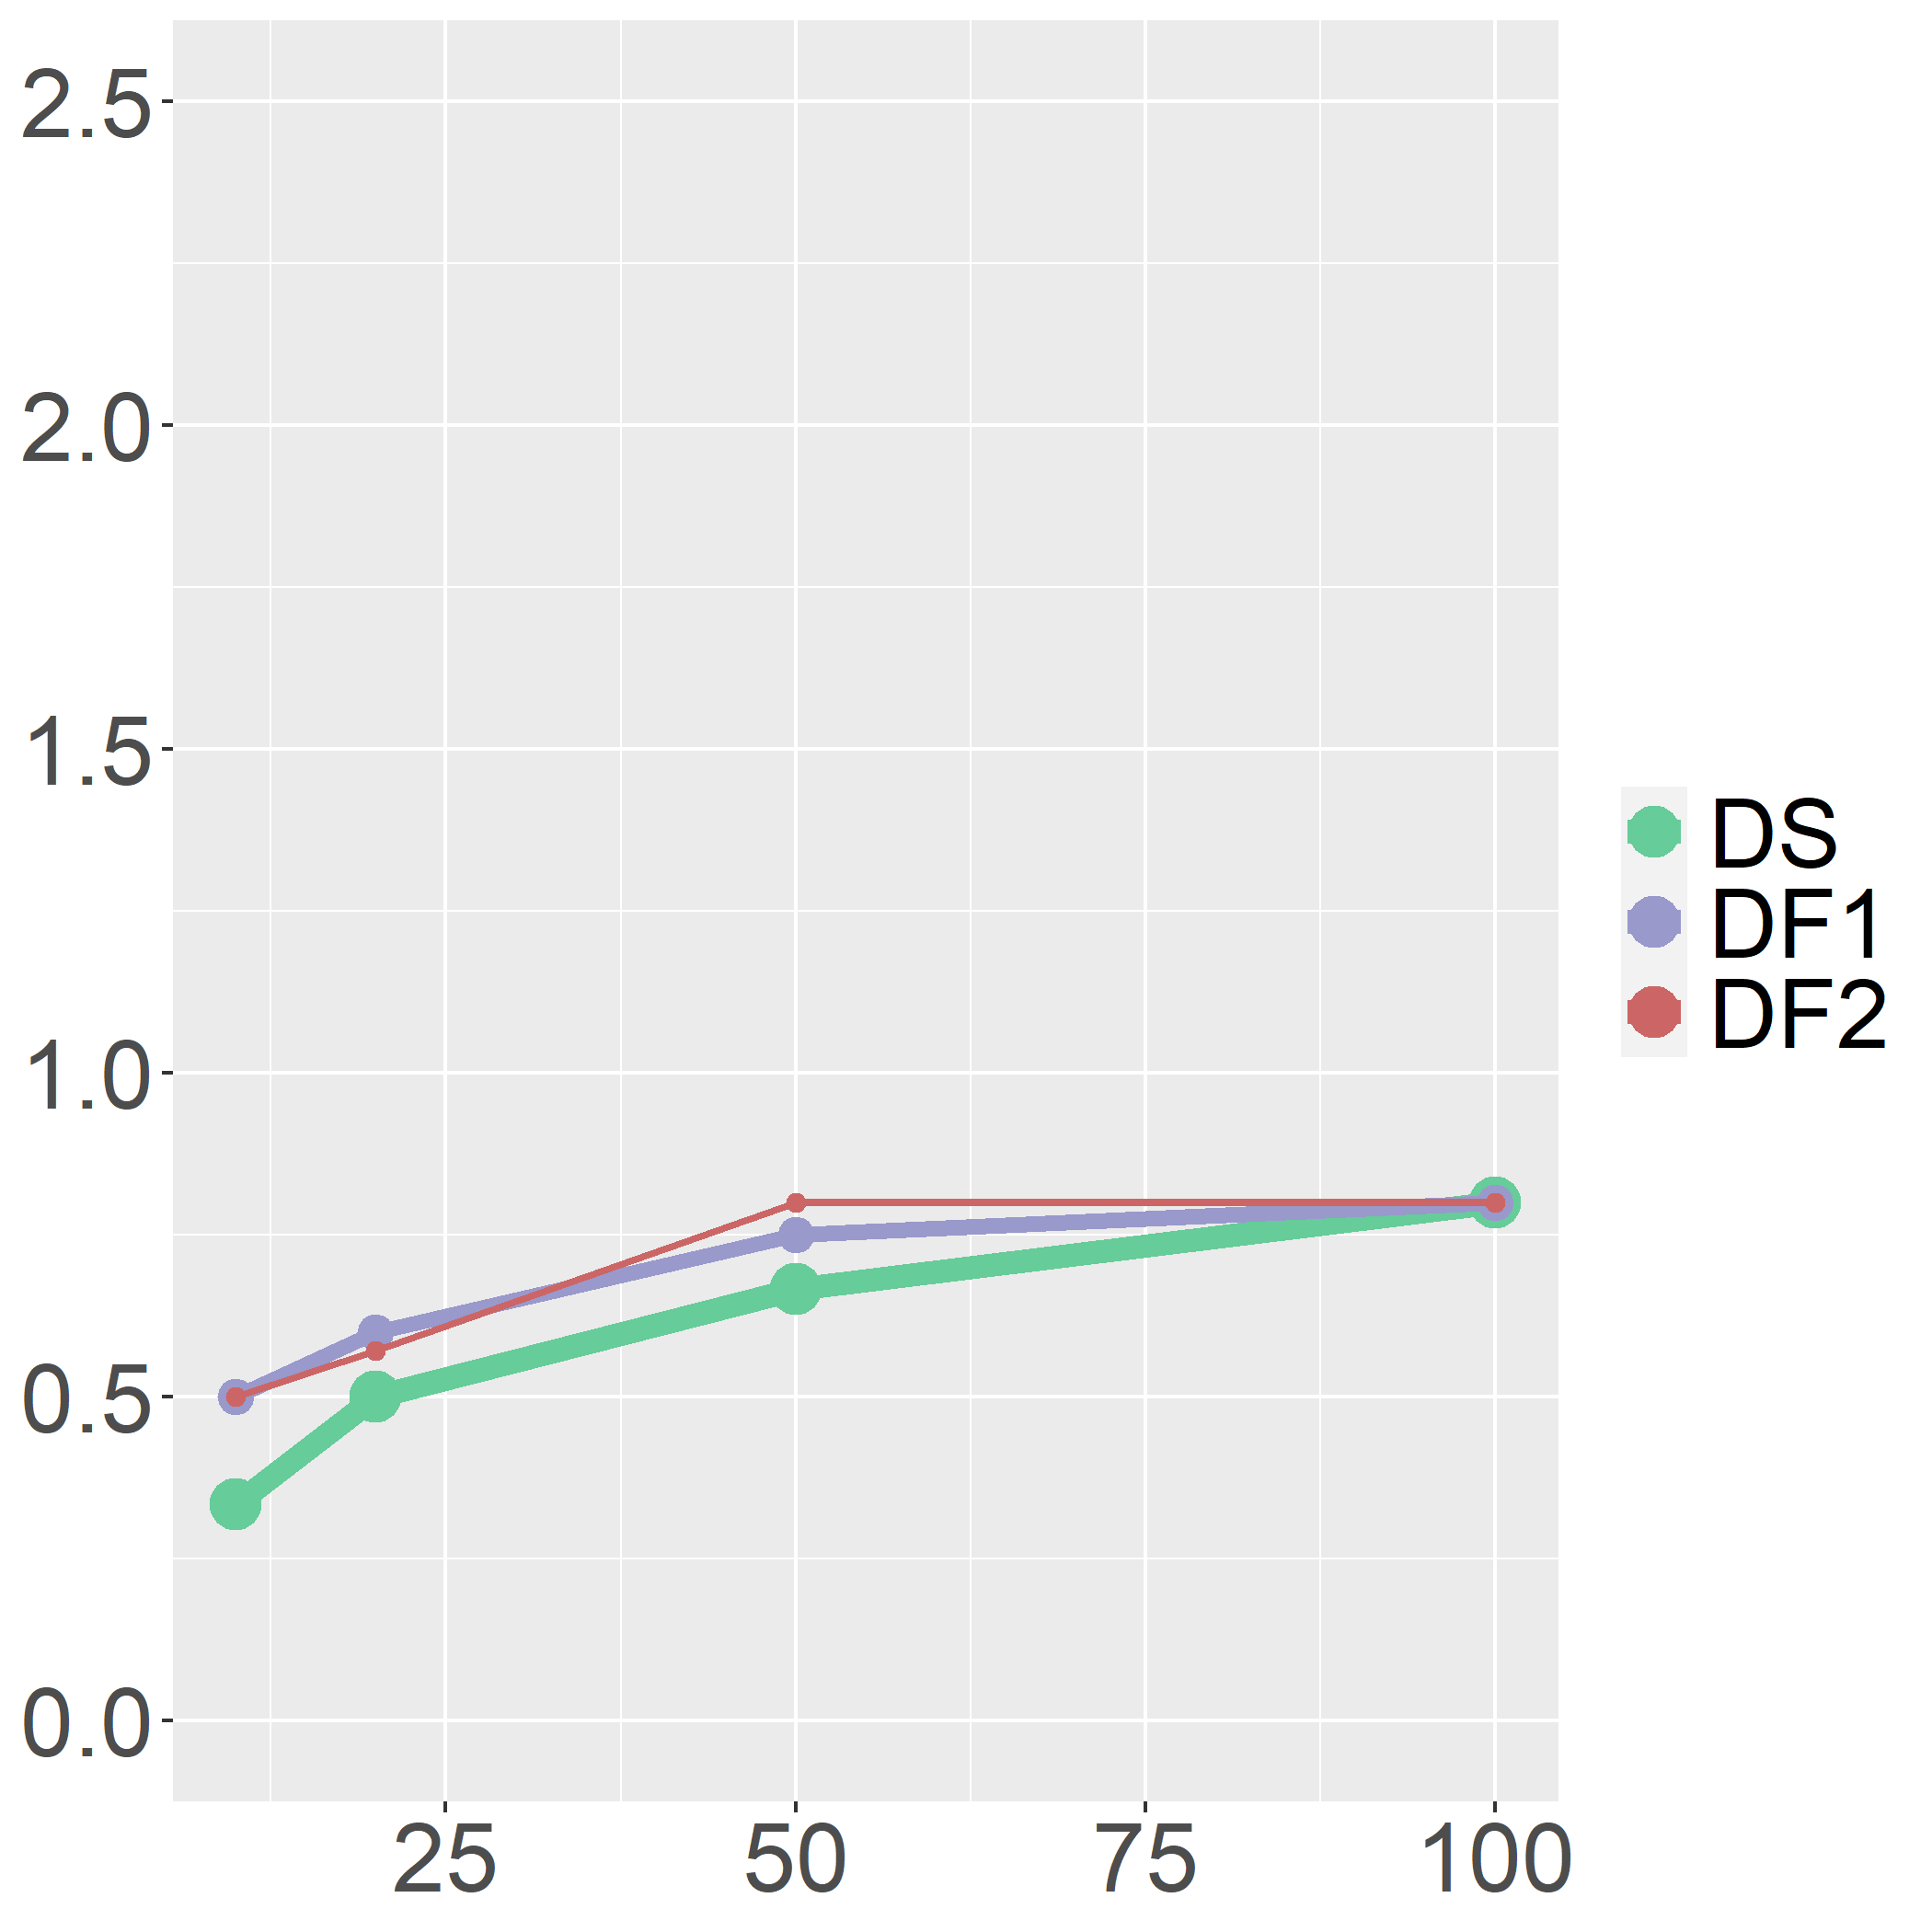
\includegraphics[width=\columnwidth]{../../plot/precision_1.png}
    \caption{(b) Precision}
    \label{fig:precision}
\end{subfigure}
\\
\centering
\begin{subfigure}[b]{.32\columnwidth} 
    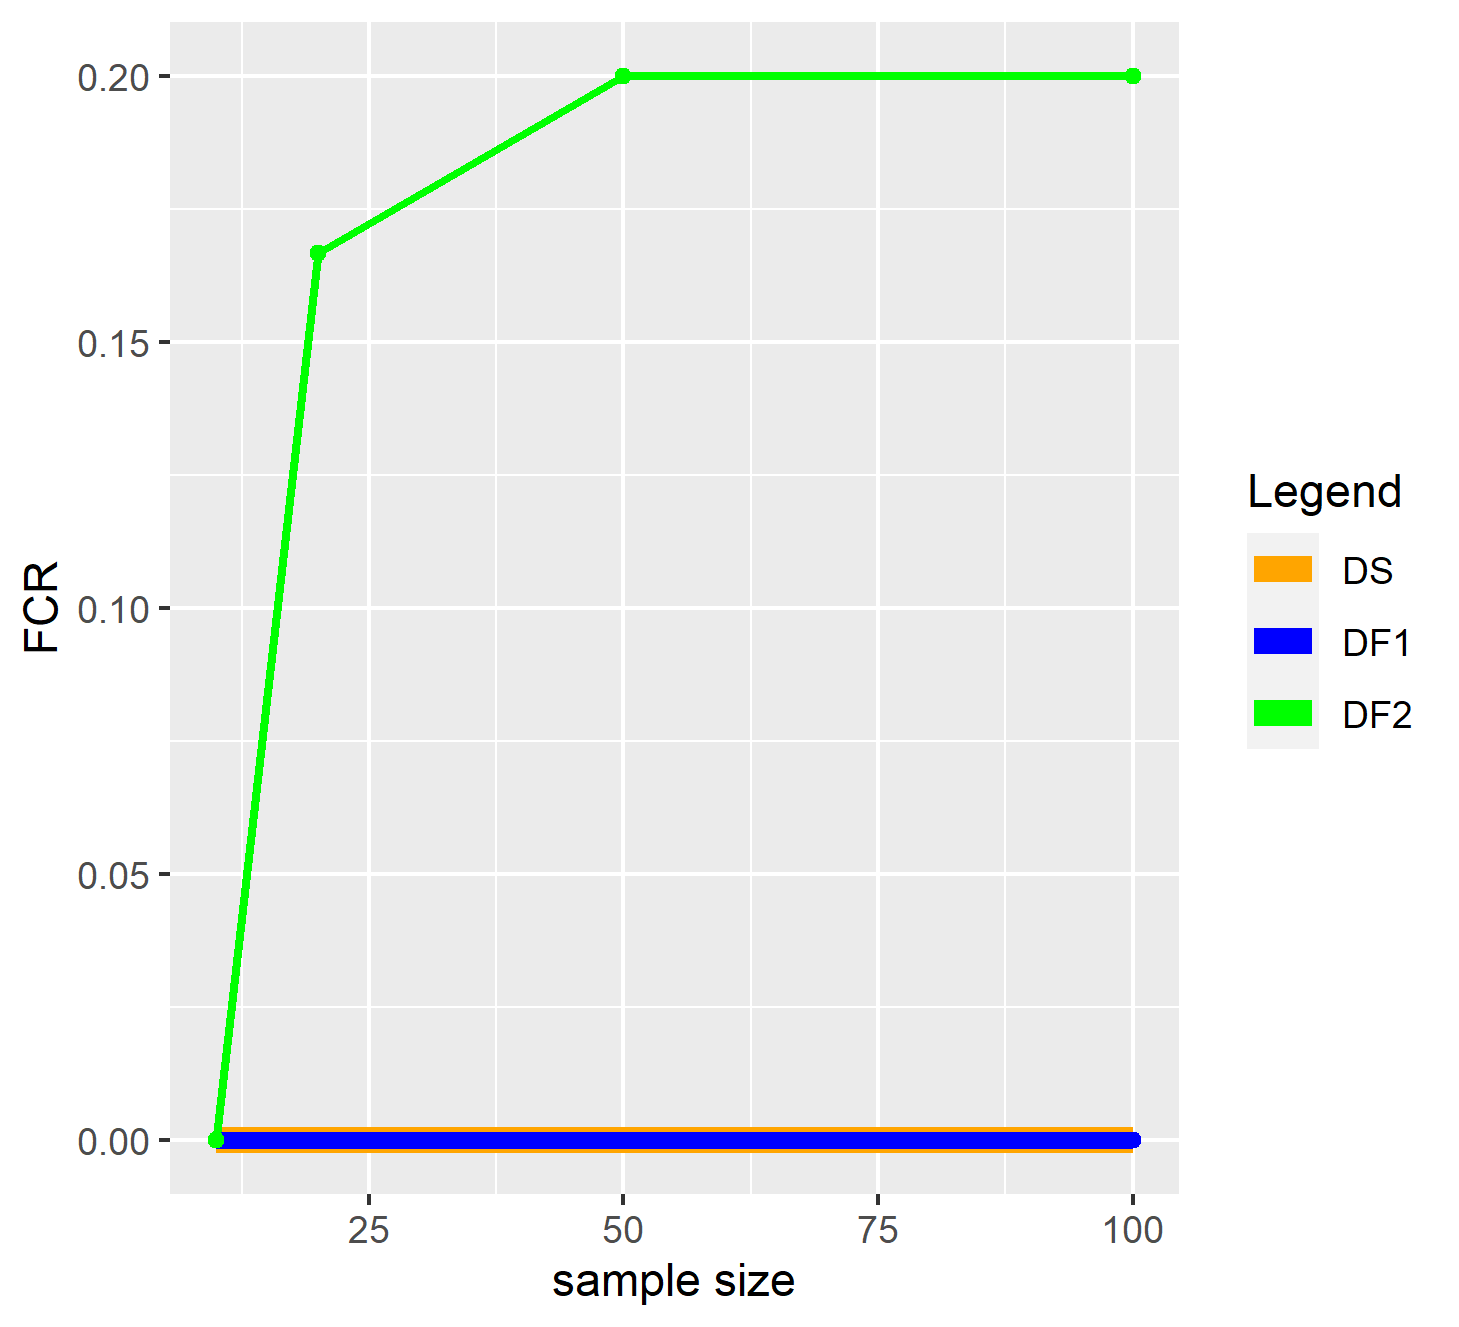
\includegraphics[width=\columnwidth]{../../plot/FCR_1.png}
    \caption{(c) FCR}
    \label{fig:fcr}
\end{subfigure}
\hfill
\centering
\begin{subfigure}[b]{.32\columnwidth} 
    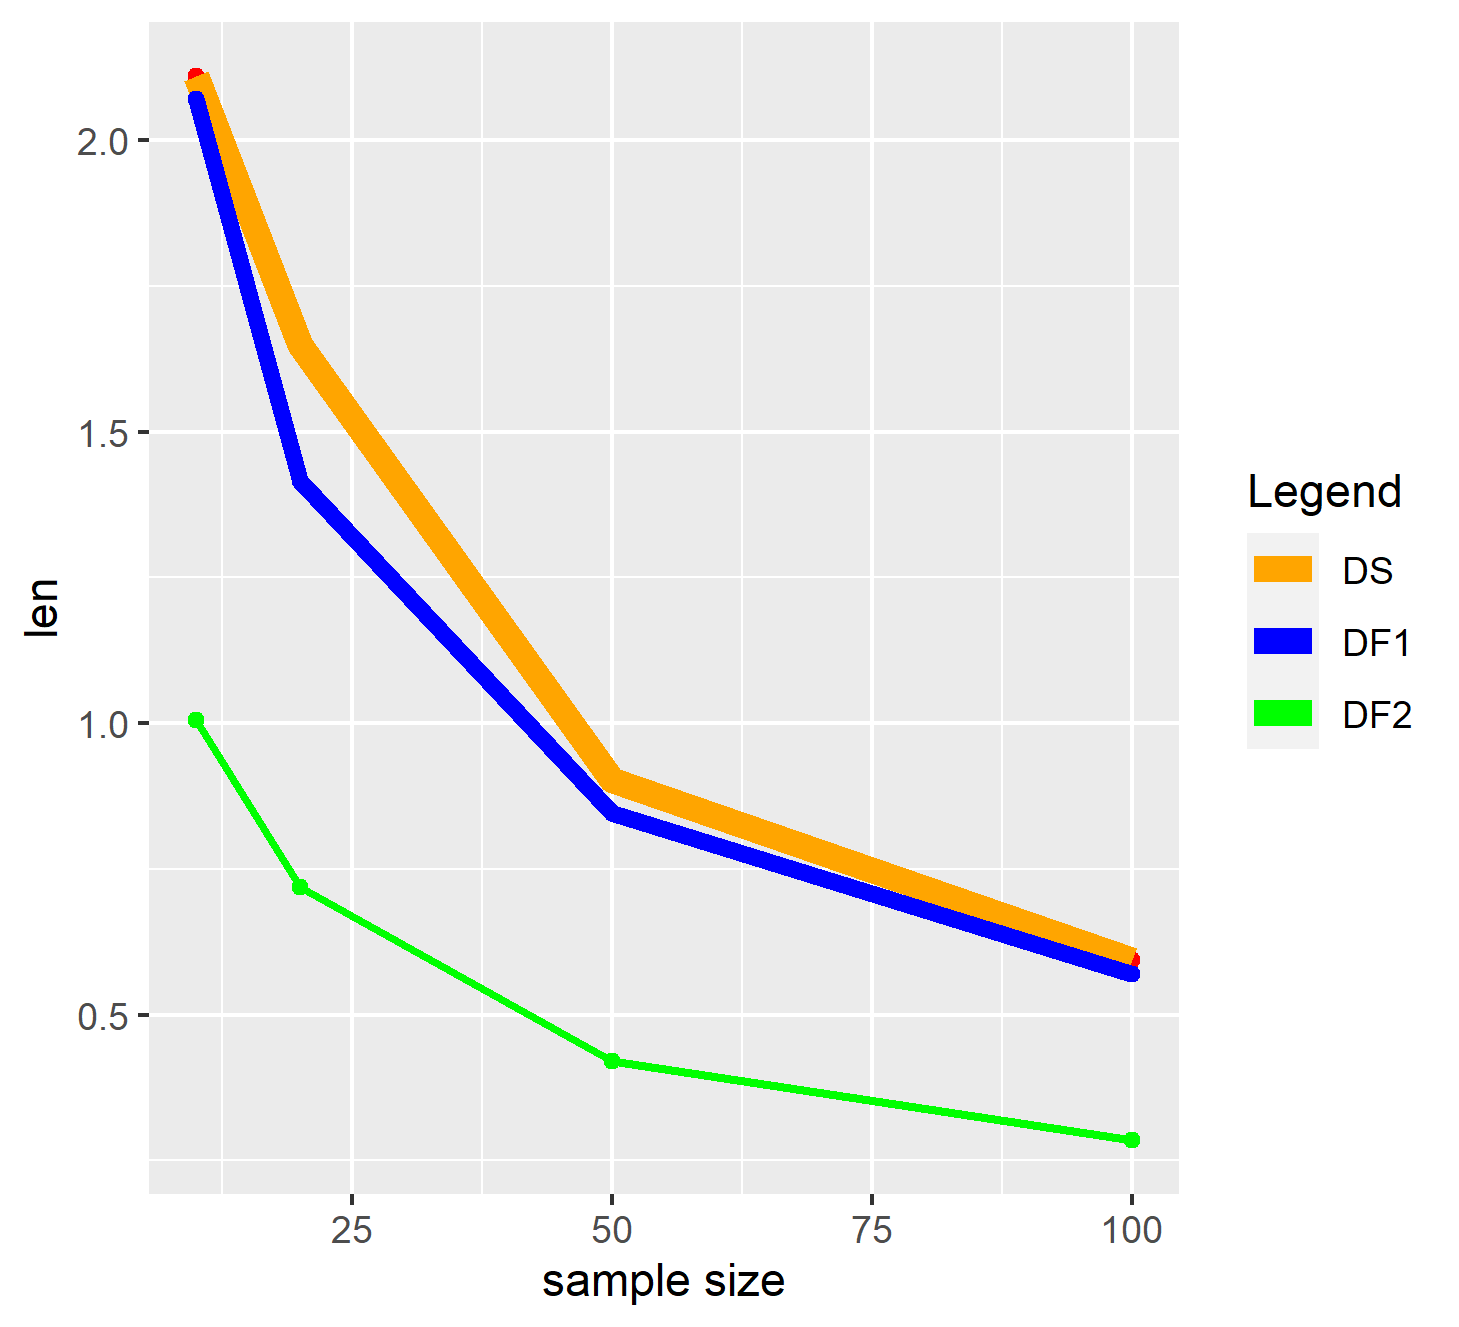
\includegraphics[width=\columnwidth]{../../plot/len_1.png}
    \caption{(d) Average CI length}
    \label{fig:ci}
\end{subfigure}
\hfill
\centering
\begin{subfigure}[b]{.32\columnwidth} 
    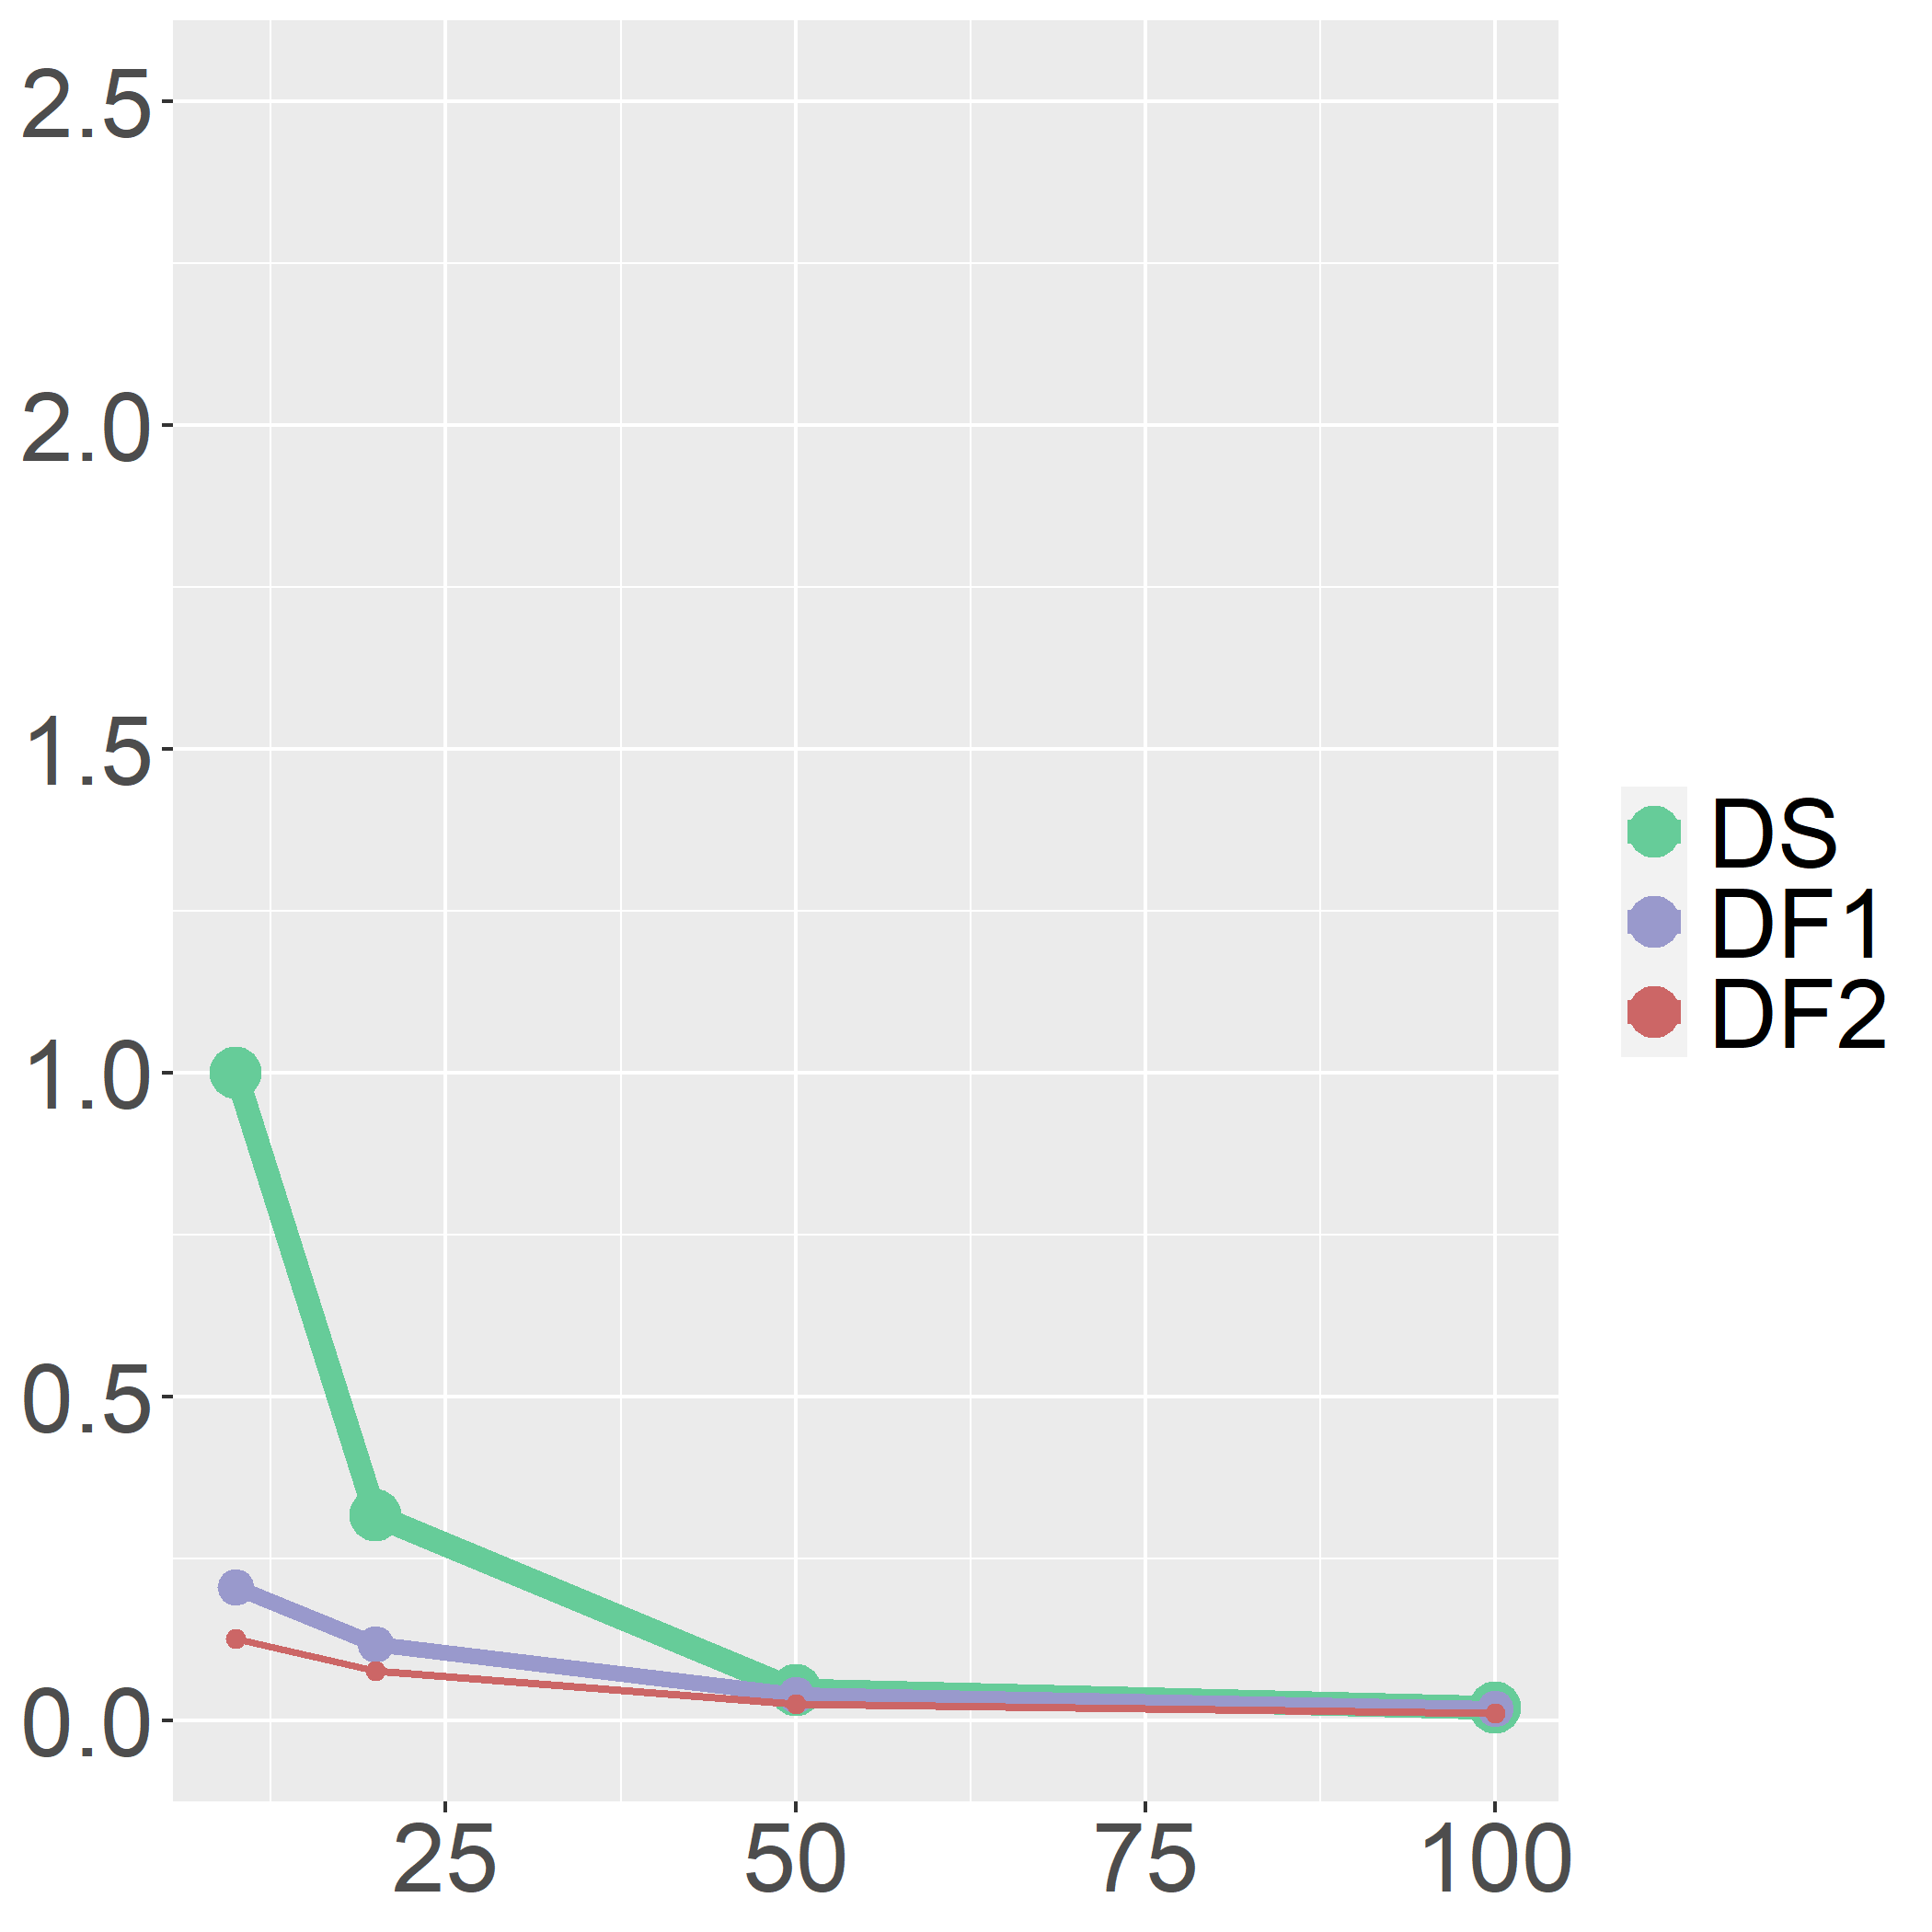
\includegraphics[width=\columnwidth]{../../plot/L2_1.png}
    \caption{(e) L2 error}
    \label{fig:l2}
\end{subfigure}
\hfill
\caption{explain what DS, DF1, DF2 stand for}
\label{fig:median}
\end{figure}

\subsection{Discussion of simulation results}

We begin by comparing variable selection accuracy through power and precision (\cref{fig:power,fig:precision}). Both metrics are similar across different sample sizes between the two data fission procedures, because they have the same $f_\tau(Y)$ marginal distributions with $\tau=1$. Compared to data splitting, data fission achieves higher power and precision, particularly when sample size is small. When there are few observations, the disadvantage of data splitting working with only half of the observations becomes apparent. In particular, if we look at individual trials (\cref{fig:split10}), data splitting tends to miss true features and pick instead many false features, leading to suboptimal power and precision. This is to be expected, as when there is not a lot of information from the data, halving the number of observations would likely hinder the quality of variable selection. Although data fission inflates the variance of the observations by a factor of two, this seems to be a worthy price to pay in order to not reduce the number of observations used in the selection stage. As we increase the sample size, however, even half of the information becomes sufficient for variable selection, which makes the advantage of data fission less obvious.

We now look at the quality of inference through FCR, avg. CI length, as well as the L2 error between the estimated parameter and the ideal target of inference averaged by the number of variables selected. \cref{fig:fcr} shows that the median FCR for data splitting and data fission (P1) are both well below the target level $\alpha = 0.05$ using standard unadjusted $95\%$ CIs. Note that no correction is needed here since the proportion of CIs covering their respective parameters is expected to be $0.95$ \citep{benjamini2005false}. On the other hand, data fission (P2) has a much higher FCR (above the target level). This is due to the mean of $\hbeta(M)$ being different than $\beta^\star(M)$ and its variance being further deflated by the fission procedure. This is evident in \cref{fig:p2_100}. Interestingly, when the sample size is small ($n=10$), data fission (P2) is also able to control the FCR. One possible explanation is that the small sample size makes $(X^\top X)^{-1}$ highly variable and thus more likely widens the corresponding CI compared to when the sample size is large. It is also worth noting that having a low FCR does not necessarily mean that we recover the true parameters, because there is a discrepancy between $\beta$ and $\beta^\star(M)$, especially when sample size is small (see for example \cref{fig:split10}).

In terms of the average length of $95\%$ CIs (\cref{fig:ci}), we see that data fission (P1) and data splitting are similar across all sample sizes. This suggests that the effect on the average length of CI is similar between inflating the variance and halving the number of observations. On the other hand, the average CI length for data fission (P2) is much smaller than the other two methods. This can be explained by that the variance of $\hbeta(M)$ is deflated by the fission procedure and that there is no reduction in sample size.

Finally, we compare the L2 error between the estimated parameter and the ideal target of inference averaged by the number of variables selected in \cref{fig:l2}. We see here that the L2 error decays as the sample size increases for all three methods. We see that the L2 error for data splitting is much higher than the two data fission procedures, particularly when the sample size is small. This is again due to data splitting reducing the sample size at the inference stage, which introduces uncertainty. It is somewhat surprising, however, to see that both data fission methods result in very similar L2 errors, despite data fission (P2) being not targeting the ideal parameter ($\EE[\hbeta(M)] \neq \beta^\star(M)$). Considering the high FCR of data fission (P2), this implies that the effect of the discrepancy between $\EE[\hbeta(M)]$ and $\beta^\star(M)$ does not hinder the inference performance as much as the deflation of $\hbeta(M)$'s variance. This calls for further investigation, and a possible way to explore this issue is to compare the L2 errors across different $\sigma^2$ values in order to amplify the effect.
\section{Discussion}
From the simulation study in the previous section, we know that in the context of constructing selective CIs in fixed-design Gaussian linear regression models, data fission (P1) outperforms data splitting, especially in the small sample setting, in both the selection and inference stage. Even with the advantage of data fission wearing off as the sample size increases, data fission (P1) still remains competitive to data splitting. This adds to Section 4 in \cite{leiner2022data}, which demonstrates that data fission (P1) can handle high leverage points better than data splitting does in the linear regression case. Therefore, if the variance of the error term ($\sigma^2$) is known, in the context of constructing selective CIs in fixed-design Gaussian linear regression models, data fission (P1) does address at least two of the shortcomings of data splitting. Namely when the sample size is small and when the data contains high leverage points. It is worth noting, however, that in our simulation study, we do not check the effect of changing (1) the data splitting ratio $a$, (2) the data fission tuning parameter $\tau$, or (3) the variance of the error term $\sigma^2$. It is important to explore the effects these three parameters have on the performance of selective inference in the given context in order to get a more comprehensive understanding of the pros and cons of data fission compared to data splitting.

On the other hand, the simulation study reveals a potentially crucial problem with the data fission (P2) procedure. Namely, by adopting the data fission (P2) procedure, we no longer target the idea parameter for inference in the linear regression case. As we have observed, this leads to a notable increase in the FCR. In fact, this procedure makes the FCR to be much higher than the target level. This raises a more general question on whether and how we can modify our corresponding selection and inference algorithm in order to accommodate cases where our inference target is different from the ideal target parameter under the data fission framework.

Finally, as briefly mentioned in \cref{sec:challenge}, the general ``conjugate prior reversal'' framework for deriving data fission procedures for distributions in the exponential family also sometimes poses challenges with regard to optimization when computing the estimated parameters in the context of constructing selective CIs in fixed-design generalized linear models. While \cite{leiner2022data} develops working solutions for when the estimated parameters are difficult to compute by changing the underlying likelihood functions, the robustness of this working solution to the modified likelihood functions remains unclear.

To summarize, there are still many important questions that need to be investigated with respect to the general ``conjugate prior reversal'' framework for deriving data fission procedures for distributions in the exponential family. Given the generality and flexibility of this data fission procedure, it is of great interest to answer these questions so that we can provide guidance when using this method in practice. Once these questions are addressed, data fission can become a preferable alternative to data splitting and data carving due to its improved performance on selective inference, as well as its wider applicability in terms of the choice of selection and inference algorithms.


\bibliographystyle{plainnat}
\bibliography{../references/qp.bib}

\end{document}
